%------------------------------------------------------------------------------
%  er-model.tex
%------------------------------------------------------------------------------
%
%	BA6 - Database systems
%
%	Authors :
%		203267 - Bastien Antoine
%		183785 - Denoréaz Thomas
%		185078 - Dieulivol David
%
%	Versions :
%		2013.03.30 - Initial version
%

\chapter{Entity–relationship model}

\begin{figure}[h!]
	\centering
	\fbox{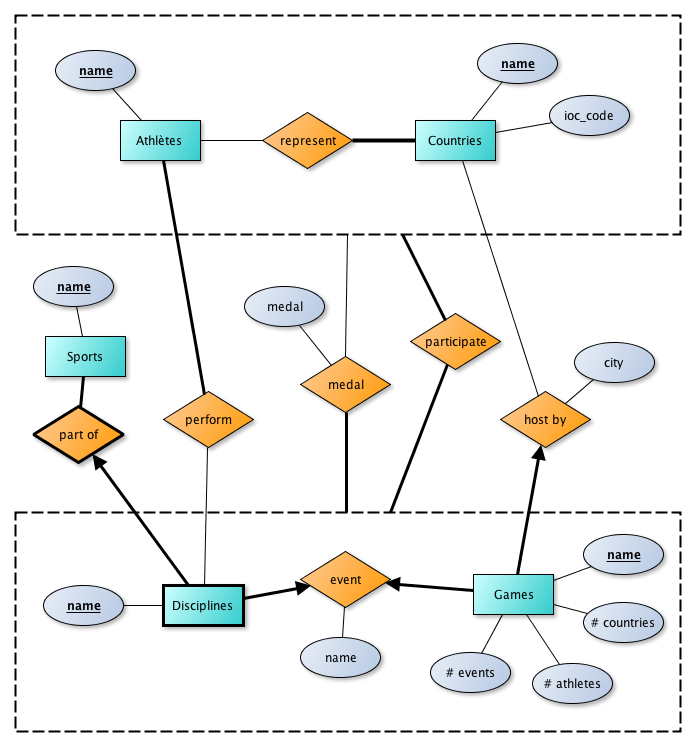
\includegraphics[width=0.5\textwidth]{er-model-old}}
	\caption{Previous ER Model.\label{fig:er-model-old}}
\end{figure}

From the analysis of the Dataset, here are our assumptions:

\begin{itemize}
	\item[$\circ$] An \textbf{Athlete} is always performing a \textbf{Discipline} instead of just a \textbf{Sport}.
	\item[$\circ$] An \textbf{Athlete} can represent only a \textbf{Country} for a \textbf{Game}. However, he can represent another \textbf{Country} for another \textbf{Game}.
	\item[$\circ$] A \textbf{Game} can only be hosted by one and only one \textbf{Country}, but this \textbf{Country} can host several \textbf{Games}.
	\item[$\circ$] Each \textbf{Discipline} is defined by its \textbf{Sport}.
	\item[$\circ$] An \textit{Event} is characterized by only a \textbf{Game} and only a \textbf{Discipline}.
	\item[$\circ$] A \textit{Medal} is obtained for a \textit{Representant} during an \textit{Event}.
	\item[$\circ$] A \textit{Participant} is formed by both a \textit{Representant} and an \textit{Event}.
\end{itemize}

\section*{Changes since deliverable 1}
After the first deliverable, we have made some simplifications to our model.
There are still two aggregations standing for a representative (\textbf{athlete} and \textbf{country}) and an event (\textbf{discipline} and \textbf{games}). These aggregations are bonded by the relation \textit{Representant\_participates\_Event} which models the participation from a representative to a \textbf{discipline}.
We have removed the other relations between them because there is only redundant information and we can put the medal attribute in the participation relation.

\begin{figure}[h!]
	\centering
	\fbox{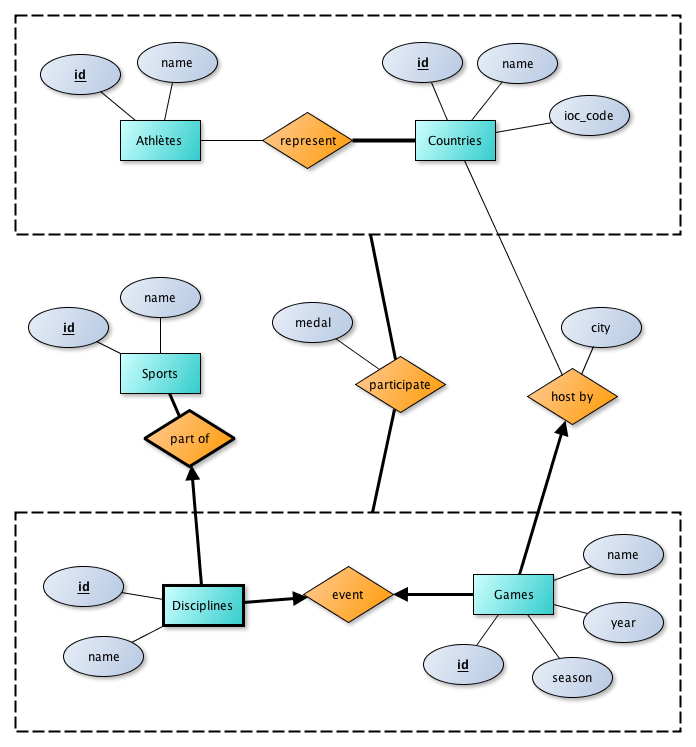
\includegraphics[width=0.8\textwidth]{er-model}}
	\caption{New ER Model.\label{fig:er-model}}
\end{figure}


%------------------------------------------------------------------------------
% END OF DOCUMENT
%------------------------------------------------------------------------------